\documentclass[11pt]{amsart}
%     If you need symbols beyond the basic set, uncomment this command.
\usepackage{amssymb}
\usepackage{amsmath}
\usepackage{mathrsfs}
\usepackage{bm}
\numberwithin{figure}{section}

%     If your article includes graphics, uncomment this command.
\usepackage{graphicx}

%     If the article includes commutative diagrams, ...
\usepackage[cmtip,all]{xy}

%     If the article includes some tikzpictures.
\usepackage{tikz}

%     Set each margin to 1in
\usepackage[margin=1in]{geometry}

%     Algorigthm
\usepackage{algpseudocode}
\usepackage{algorithmicx,algorithm}

%     Define theorem, definition, example, exercise, equation and remak environments
\theoremstyle{plain}
\newtheorem{theorem}{Theorem}[section]
\theoremstyle{definition}
\newtheorem{lemma}[theorem]{Lemma}
\newtheorem{defi}[theorem]{Definition}
\newtheorem{xca}[theorem]{Exercise}
\newtheorem{sol}[theorem]{Solution}
\newtheorem*{remark}{Remark}
\numberwithin{equation}{section}

%    Blank box placeholder for figures (to avoid requiring any
%    particular graphics capabilities for printing this document).
\newcommand{\blankbox}[2]{%
  \parbox{\columnwidth}{\centering
%    Set fboxsep to 0 so that the actual size of the box will match the
%    given measurements more closely.
    \setlength{\fboxsep}{0pt}%
    \fbox{\raisebox{0pt}[#2]{\hspace{#1}}}%
  }%
}

%    To combine rows in talbe
\usepackage{multirow}

%    Generating simple two- and three-set Venn diagrams 
\usepackage{venndiagram}

%    Set itemize 
\usepackage{enumitem}
\setenumerate[1]{leftmargin=2em,itemsep=0pt,partopsep=0pt,parsep=\parskip,topsep=5pt}
\setitemize[1]{leftmargin=2em,itemsep=0pt,partopsep=0pt,parsep=\parskip,topsep=5pt}
\setdescription[1]{leftmargin=2em,itemsep=0pt,partopsep=0pt,parsep=\parskip,topsep=5pt}

%    Private Package
\usepackage{examplepackage}

%    body
\begin{document}
 
%    Set noindent for entire file
\pagestyle{plain}

%    Set parskip for entire file
\setlength\parskip{1em}

%    Information for title
\title{}

%    Information for author
\author{}

\date{}

% \maketitle

\section{Constitutive models of materials}
\subsection{Starin measures}
Assume cell wall is a smooth surface $S \subset \mathbf{R}^{3} $, $\bm{n}$ is the exterior normal vector to $S$.
Define the deformation is $\bm{u} \in \mathbf{H}^{1} (S)$, 
its gradient is denoted by $ \mathbb{F} := \nabla \bm{u}$.
\textbf{Green-Lagrangian strain tensor} is defined by 
\[
  \mathbb{E} = \frac{1}{ 2 } \left(\mathbb{F}^{\top} \mathbb{F} - \mathbb{I}\right).
\]
The Green strain succeeds in discarding the rotational degrees of freedom,
which have no bearing on the serverity of deformation, 
and retains the stretch/shear information in the 6-DOF symmetric factor.
We can construct a \textbf{linear} approximation by forming a Taylor expansion around the undeformed configuration $\mathbb{F} = \mathbb{I}$.
\[
  \mathbb{E} \left(\mathbb{F}\right) \approx 
  \mathbb{E} \left(\mathbb{I}\right) + 
  \frac{ \partial \mathbb{E} }{ \partial \mathbb{F} } 
  \big\rvert_{\mathbb{F} = \mathbb{I}} : 
  \left(\mathbb{F} - \mathbb{I}\right) 
  = 
  \frac{ \partial \mathbb{E} }{ \partial \mathbb{F} } 
  \big\rvert_{\mathbb{F} = \mathbb{I}} : 
  \left(\mathbb{F} - \mathbb{I}\right),
\] 
where $:$ is the double dot product defined by $\mathbb{A}:\mathbb{B} = \text{tr}(\mathbb{A}^{\top} \mathbb{B})$.
The derivative $\partial \mathbb{E} / \partial \mathbb{F}$ is most conveniently defined via the differetial $\delta \mathbb{E}$ :
\[
  \frac{ \partial \mathbb{E} }{ \partial \mathbb{F} } : 
  \delta \mathbb{F}
  =  \delta \mathbb{E}
  = \frac{1}{ 2 } \left( \delta \mathbb{F}^{\top} \mathbb{F} +
  \mathbb{F}^{\top} \delta \mathbb{F}\right) .
\] 
Thus 
\[
  \frac{ \partial \mathbb{E}}{ \partial \mathbb{F}} 
  \big \rvert_{\mathbb{F} = \mathbb{I} }  : 
  \left(\mathbb{F} - \mathbb{I}\right) = 
  \frac{ 1 }{ 2 } \left[ 
    \left(\mathbb{F} - \mathbb{I}\right)^{\top} \mathbb{I} + 
    \mathbb{I}^{\top} \left(\mathbb{F} - \mathbb{I}\right)
  \right]
  = \frac{ 1 }{ 2 } \left(
    \mathbb{F}^{\top} + \mathbb{F}
  \right) - \mathbb{I}.
\] 
The matrix resulting from this linear approximation of $\mathbb{E}(\mathbb{F})$ is denoted by $\bm{\epsilon}$, where:
\[
  \bm{\epsilon} = \frac{ 1 }{ 2 } \left(\mathbb{F}^{\top} + \mathbb{F}\right) - \mathbb{I}
\] 
and called the \textbf{small strain tensor}, or the 
\textbf{infinitesimal strain tensor}.

\subsection{linear elasticity}
The simplest practical constitutive model is \textbf{linear elasticity}, 
defined in terms of the strain energy density as: 
\[
  \Psi \left(\mathbb{F}\right) = 
  \mu \bm{\epsilon} : \bm{\epsilon} 
  + \frac{ \lambda }{ 2 } \text{tr} ^{2} \left(\bm{\epsilon}\right),
\] 
where $\bm{\epsilon}$ is the small strain tensor, 
and $\mu, \lambda$ are the \textbf{Lam\'e coefficients}, 
which are related to the material properties of  \textbf{Young's modulus} $k$ (a measure of stretch resistance) and \textbf{Poisson's ratio} $\nu$ (a measure of incompressibility) as:
\[
\mu = \frac{ k }{ 2 \left(1+\nu\right) } \quad 
\lambda = \frac{ k \nu }{ \left(1+\nu\right) \left(1 - 2\nu\right) } .
\] 
The relation between the  \textbf{first Piola stress} $\mathbb{P}$ and $\mathbb{F}$ can be derivaed as follows:
\[
  \mathbb{P} = \frac{ \delta \Psi }{ \delta \mathbb{F} }  = 
  2 \mu \bm{\epsilon} + \lambda \text{tr} \left(\bm{\epsilon}\right) \mathbb{I},
\] 
or, after one final substitution for $\bm{\epsilon}$ (and a few algebraic reductions):
\[
  \mathbb{P} \left(\mathbb{F}\right) = 
  \mu \left(\mathbb{F} + \mathbb{F}^{\top} - 2 \mathbb{I}\right) 
  + \lambda \text{tr} \left(\mathbb{F} - \mathbb{I}\right) \mathbb{I}.
\] 
In the Voigt matrix form, the above relation can be written as 
\[
\left[
\begin{array}{c}
\mathbb{P}_{11} \\
\mathbb{P}_{22} \\
\mathbb{P}_{33} \\
\mathbb{P}_{23} \\
\mathbb{P}_{13} \\
\mathbb{P}_{12} \\
\end{array}
\right] 
= 
\left[
\begin{array}{cccccc}
2 \mu + \lambda & \lambda & \lambda & 0 & 0 & 0 \\
\lambda & 2 \mu + \lambda & \lambda & 0 & 0 & 0 \\
\lambda & \lambda & 2 \mu + \lambda & 0 & 0 & 0 \\
0 & 0 & 0 & \mu & 0 & 0 \\
0 & 0 & 0 & 0 & \mu & 0 \\
0 & 0 & 0 & 0 & 0 & \mu \\
\end{array}
\right]
\left[
\begin{array}{c}
\bm{\epsilon}_{11} \\
\bm{\epsilon}_{22} \\
\bm{\epsilon}_{33} \\
2\bm{\epsilon}_{23} \\
2\bm{\epsilon}_{13} \\
2\bm{\epsilon}_{12} \\
\end{array}
\right] 
\] 
where the transition matrix in the above equality can written as:
\[
\frac{ k }{ \left(1+\nu\right) \left(1-2\nu\right) } 
\left[
\begin{array}{cccccc}
1 - \nu & \nu & \nu & 0 & 0 & 0 \\
\nu & 1 - \nu & \nu & 0 & 0 & 0 \\
\nu & \nu & 1 - \nu & 0 & 0 & 0 \\
0 & 0 & 0 & \frac{ 1-2\nu }{2 }  & 0 & 0 \\
0 & 0 & 0 & 0 & \frac{ 1-2\nu }{ 2 }  & 0 \\
0 & 0 & 0 & 0 & 0 & \frac{ 1-2\nu }{ 2 }  \\
\end{array}
\right]
\] 

\subsection{The PDE form of linear elasticity}
Assume an externally applied force distribution $\bm{f}_{\rm ext} $.
When the object has settled to an equilibrium (rest) configuration, the deformation function will satisfy: 
\begin{align}
  \text{div} \mathbb{P}  = \bm{f}_{\rm ext},  
\end{align}
which can lead to the following formulation:
\begin{align}
  - \mu \Delta \bm{u} 
  - \left(\mu + \lambda\right) \nabla 
  \left( \text{div} \bm{u} \right) 
  = \bm{f}_{\rm ext} .
\end{align}

Numerical experiments:
\begin{figure}[!tbh]
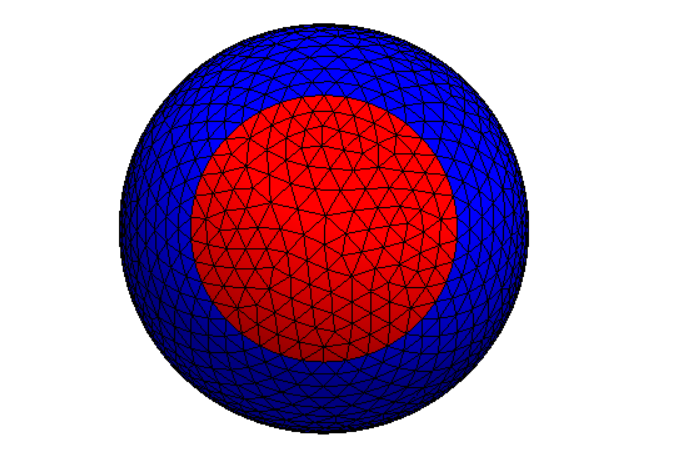
\includegraphics[width=3in]{./figures/k.png}
\end{figure}

\[
\nu = 0.5, 
k = 
\begin{cases}
1 \quad \text{in}\quad \text{CZ},\\
0.25 \quad \text{in} \quad \text{PZ},
\end{cases}
\bm{f} = 0.2 \bm{n}.
\] 



\begin{figure}
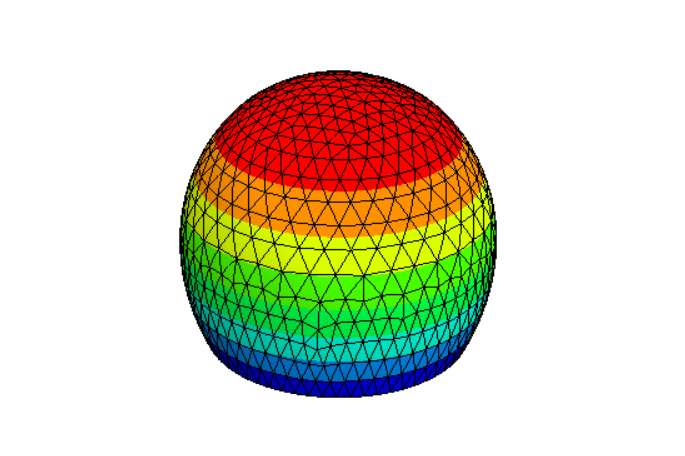
\includegraphics[width=4in]{./figures/deform.png}
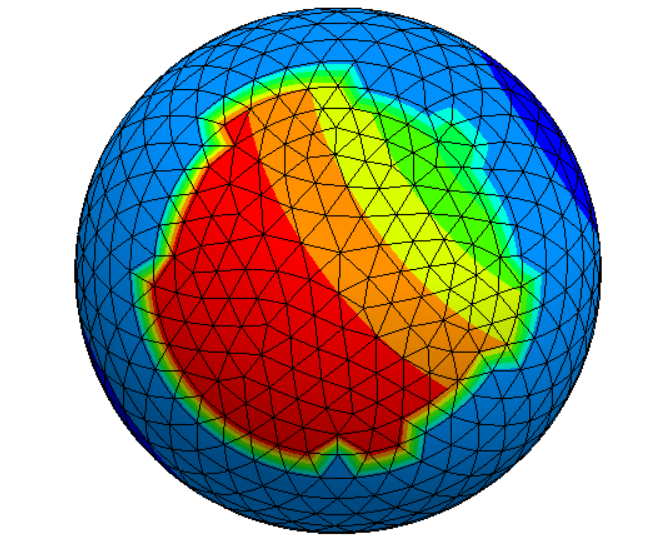
\includegraphics[width=3in]{./figures/surfa.png}
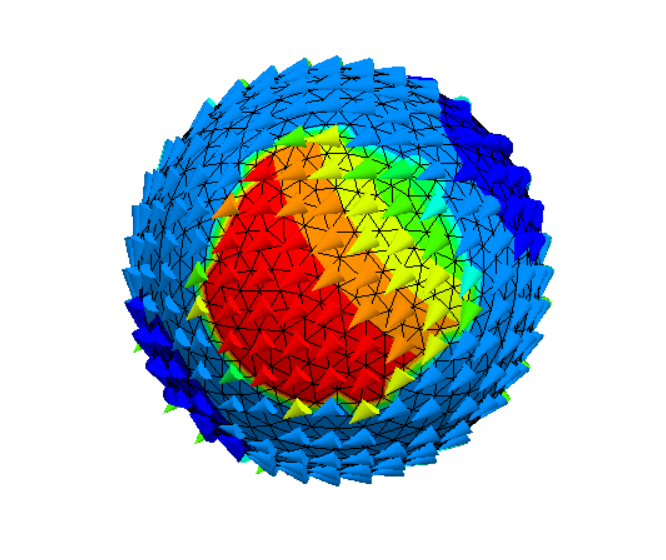
\includegraphics[width=3.5in]{./figures/surfv.png}
\end{figure}



%% end of subsection{The PDE of linear elasticity}



\end{document}
